\documentclass[t]{beamer}
\usetheme{Copenhagen}
\setbeamertemplate{headline}{} % remove toc from headers
\beamertemplatenavigationsymbolsempty

\usepackage{amsmath, array, tikz, bm, pgfplots, tcolorbox, graphicx, venndiagram, color, colortbl, xfrac}
\pgfplotsset{compat = 1.16}
\usepgfplotslibrary{statistics}
\usetikzlibrary{calc}

\title{Scatterplots and Correlation}
\author{}
\date{}

\AtBeginSection[]
{
  \begin{frame}
    \frametitle{Objectives}
    \tableofcontents[currentsection]
  \end{frame}
}

\begin{document}

\begin{frame} 
\maketitle
\end{frame}

% Create scatterplots
\section{Create and analyze scatterplots}

\begin{frame}{Scatterplots}
\begin{tcolorbox}[colframe=green!20!black, colback = green!30!white,title=\textbf{Scatterplot}]
A \textbf{scatterplot} is a visual display which can be used to examine an association between two variables, usually $x$ and $y$.
\end{tcolorbox}
\bigskip	\pause

The independent variable, $x$, is called the {\color{blue}\textbf{explanatory variable}} and the dependent variable, $y$, is called the {\color{blue}\textbf{response variable}}.	\bigskip	\pause

Scatterplots allow us to see if there is a relationship between the two variables.
\end{frame}

\begin{frame}{Example 1}
The table below shows the age of a certain model of car (in years) with the cars current value (in thousands of dollars). Create a scatterplot for the data.	\newline\\
\begin{minipage}{0.3\textwidth}
\scalebox{0.9}{
\begin{tabular}{c|c}
\textbf{Age} & \textbf{Value} \\ \hline
2 & 15 	\\
3 & 12	\\
3 & 13	\\
2 & 14	\\
4 & 13	\\
5 & 10	\\
6 & 10.5	\\
1 & 16.5	\\
0 & 18		\\
4 & 14		\\
7 & 11		\\
\end{tabular}}
\end{minipage}
\hspace{0.25cm}
\onslide<2->{
\begin{minipage}{0.6\textwidth}
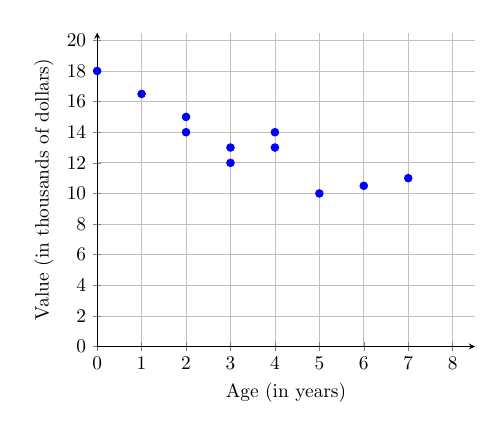
\begin{tikzpicture}[scale=0.7]
	\begin{axis}[
	axis lines = left, grid,
	xlabel = {Age (in years)},
	ylabel = {Value (in thousands of dollars)},
	xmin = 0, xmax = 8.5,
	ymin = 0, ymax = 20.5,
	xtick = {0,1,...,8},
	ytick = {0,2,...,20}
	]
	\addplot [only marks, color=blue] coordinates {
		(2,15)
		(3,12)
		(3,13)
		(2,14)
		(4,13)
		(5,10)
		(6,10.5)
		(1,16.5)
		(0,18)
		(4,14)
		(7,11)
	};
	\end{axis}
\end{tikzpicture}
\end{minipage}}
\end{frame}

\section{Determine the type of correlation of a scatterplot}

\begin{frame}{Direction of Points}
Often times, the data in a scatterplot has some pattern to it. \newline\\	\pause

\begin{tcolorbox}[colframe=green!20!black, colback = green!30!white,title=\textbf{Correlation}]
A \textbf{correlation} between two variables examines how the response variable's ($y$) values change as the explanatory variable's ($x$) values change.
\end{tcolorbox}
\bigskip \pause

We will examine three correlation types: positive, negative, and none (a.k.a. no correlation)
\end{frame}

\begin{frame}{Positive Correlation}
As $x$ increases, so does $y$.	\newline\\	\pause
\begin{center}
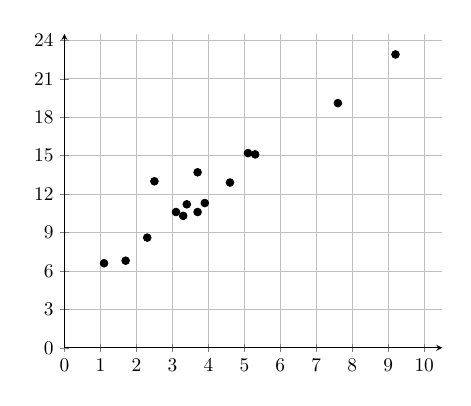
\begin{tikzpicture}[scale=0.7]
	\begin{axis}[
	axis lines = left, grid,
	%xlabel = {Age (in years)},
	%ylabel = {Value (in thousands of dollars)},
	xmin = 0, xmax = 10.5,
	ymin = 0, ymax = 24.5,
	xtick = {0,1,...,10},
	ytick = {0,3,...,24}
	]
\addplot [only marks] coordinates {
(7.6, 19.1)
(9.2, 22.9)
(3.3, 10.3)
(1.1, 6.6)
(3.7, 10.6)
(3.9, 11.3)
(4.6, 12.9)
(2.3, 8.6)
(5.1, 15.2)
(5.3, 15.1)
(2.5, 13)
(3.4, 11.2)
(3.1, 10.6)
(1.7, 6.8)
(3.7, 13.7)
};
\end{axis}
\end{tikzpicture}
\end{center}
\end{frame}

\begin{frame}{Quadrants from Means}
We can also get a \emph{general idea} of the type of correlation by looking at the counts of observations in the quadrants formed by the means of $x$ and $y$.	\newline\\		\pause
\begin{minipage}{0.6\textwidth}
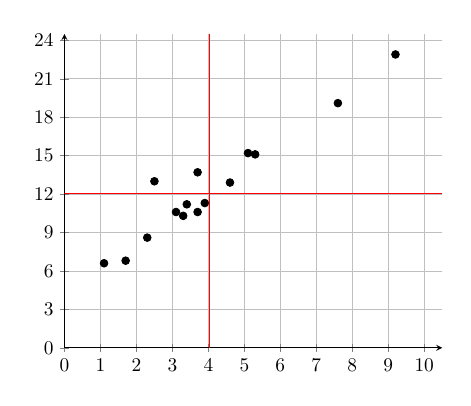
\begin{tikzpicture}[scale=0.7]
	\begin{axis}[
	axis lines = left, grid,
	%xlabel = {Age (in years)},
	%ylabel = {Value (in thousands of dollars)},
	xmin = 0, xmax = 10.5,
	ymin = 0, ymax = 24.5,
	xtick = {0,1,...,10},
	ytick = {0,3,...,24}
	]
\addplot [only marks] coordinates {
(7.6, 19.1)
(9.2, 22.9)
(3.3, 10.3)
(1.1, 6.6)
(3.7, 10.6)
(3.9, 11.3)
(4.6, 12.9)
(2.3, 8.6)
(5.1, 15.2)
(5.3, 15.1)
(2.5, 13)
(3.4, 11.2)
(3.1, 10.6)
(1.7, 6.8)
(3.7, 13.7)
};
\draw [color=red] (axis cs: 4.03,24.5) -- (4.03,0);
\draw [color=red] (axis cs: 10.5,12.09) -- (0,12.09);
\end{axis}
\end{tikzpicture}
\end{minipage}
\hspace{0.25cm}
\begin{minipage}{0.3\textwidth}
\onslide<3->{Q1: 5 values \\
Q3: 8 values \\
Total = 13} \newline\\ 
\onslide<4->{Q2: 2 values \\
Q4: 0 values \\
Total: 2} \newline\\	
\onslide<5->{11 more points in Q1 and Q3}	\\
\onslide<6->{suggests positive correlation}
\end{minipage}
\end{frame}

\begin{frame}{Negative Correlation}
As $x$ increases, $y$ decreases.	\newline\\	\pause
\begin{center}
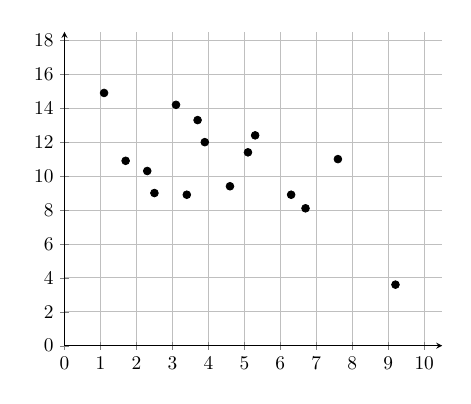
\begin{tikzpicture}[scale=0.7]
	\begin{axis}[
	axis lines = left, grid,
	%xlabel = {Age (in years)},
	%ylabel = {Value (in thousands of dollars)},
	xmin = 0, xmax = 10.5,
	ymin = 0, ymax = 18.5,
	xtick = {0,1,...,10},
	ytick = {0,2,...,18}
	]
\addplot [only marks] coordinates{
(7.6, 11.0)
(9.2, 3.6)
(6.3, 8.9)
(1.1, 14.9)
(6.7, 8.1)
(3.9, 12.0)
(4.6, 9.4)
(2.3, 10.3)
(5.1, 11.4)
(5.3, 12.4)
(2.5, 9.0)
(3.4, 8.9)
(3.1, 14.2)
(1.7, 10.9)
(3.7, 13.3)
};
\end{axis}
\end{tikzpicture}
\end{center}
\end{frame}

\begin{frame}{Quadrants from Means}
\begin{minipage}{0.6\textwidth}
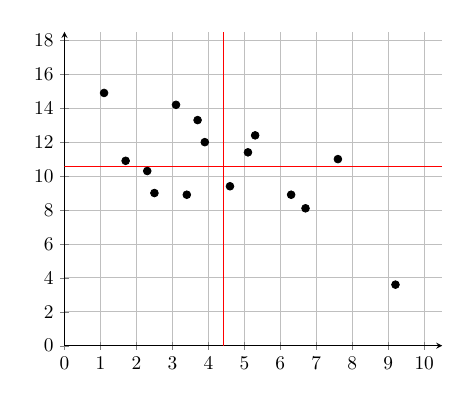
\begin{tikzpicture}[scale=0.7]
	\begin{axis}[
	axis lines = left, grid,
	%xlabel = {Age (in years)},
	%ylabel = {Value (in thousands of dollars)},
	xmin = 0, xmax = 10.5,
	ymin = 0, ymax = 18.5,
	xtick = {0,1,...,10},
	ytick = {0,2,...,18}
	]
\addplot [only marks] coordinates{
(7.6, 11.0)
(9.2, 3.6)
(6.3, 8.9)
(1.1, 14.9)
(6.7, 8.1)
(3.9, 12.0)
(4.6, 9.4)
(2.3, 10.3)
(5.1, 11.4)
(5.3, 12.4)
(2.5, 9.0)
(3.4, 8.9)
(3.1, 14.2)
(1.7, 10.9)
(3.7, 13.3)
};
\draw [color=red] (axis cs: 4.43,0) -- (axis cs: 4.43,18.5);
\draw [color=red] (axis cs: 0,10.6) -- (axis cs: 10.5,10.6);
\end{axis}
\end{tikzpicture}
\end{minipage}
\hspace{0.25cm}
\begin{minipage}{0.3\textwidth}
\onslide<2->{Q1: 3 values \\
Q3: 3 values \\
Total = 6} \newline\\ 
\onslide<3->{Q2: 5 values \\
Q4: 4 values \\
Total: 9} \newline\\	
\onslide<4->{3 more points in Q2 and Q4}	\\
\onslide<5->{suggests a very weak negative correlation}
\end{minipage}
\end{frame}

\begin{frame}{No Correlation}
There is no visible pattern between $x$ and $y$.	\newline\\	\pause
\begin{center}
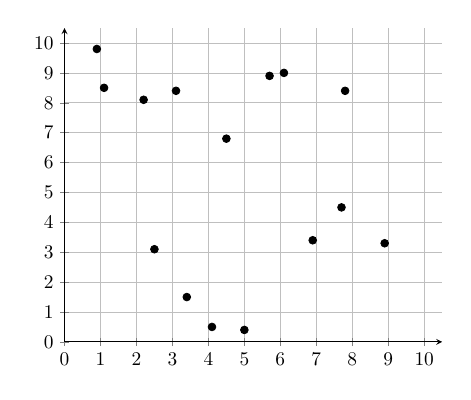
\begin{tikzpicture}[scale=0.7]
	\begin{axis}[
	axis lines = left, grid,
	%xlabel = {Age (in years)},
	%ylabel = {Value (in thousands of dollars)},
	xmin = 0, xmax = 10.5,
	ymin = 0, ymax = 10.5,
	xtick = {0,1,...,10},
	ytick = {0,1,...,10}
	]
\addplot [only marks] coordinates{
(6.9, 3.4)
(7.7, 4.5)
(0.9, 9.8)
(3.4, 1.5)
(8.9, 3.3)
(5.7, 8.9)
(3.1, 8.4)
(2.2, 8.1)
(4.5, 6.8)
(4.1, 0.5)
(5.0, 0.4)
(7.8, 8.4)
(2.5, 3.1)
(6.1, 9.0)
(1.1, 8.5)
};
\end{axis}
\end{tikzpicture}
\end{center}
\end{frame}

\begin{frame}{Quadrants of Means}
\begin{minipage}{0.6\textwidth}
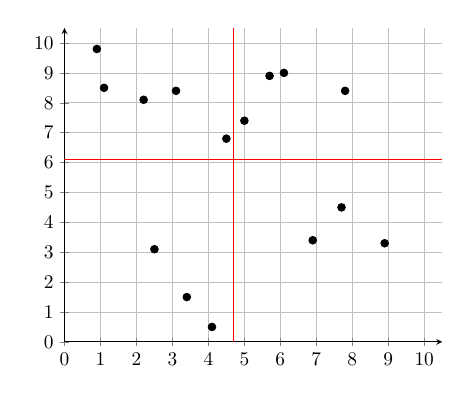
\begin{tikzpicture}[scale=0.7]
	\begin{axis}[
	axis lines = left, grid,
	%xlabel = {Age (in years)},
	%ylabel = {Value (in thousands of dollars)},
	xmin = 0, xmax = 10.5,
	ymin = 0, ymax = 10.5,
	xtick = {0,1,...,10},
	ytick = {0,1,...,10}
	]
\addplot [only marks] coordinates{
(6.9, 3.4)
(7.7, 4.5)
(0.9, 9.8)
(3.4, 1.5)
(8.9, 3.3)
(5.7, 8.9)
(3.1, 8.4)
(2.2, 8.1)
(4.5, 6.8)
(4.1, 0.5)
(5.0, 7.4)
(7.8, 8.4)
(2.5, 3.1)
(6.1, 9.0)
(1.1, 8.5)
};
\draw [color=red] (axis cs: 4.7,0) -- (axis cs: 4.7,10.5);
\draw [color=red] (axis cs: 0,6.1) -- (axis cs: 10.5,6.1);
\end{axis}
\end{tikzpicture}
\end{minipage}
\hspace{0.25cm}
\begin{minipage}{0.3\textwidth}
\onslide<2->{Q1: 4 values \\
Q3: 3 values \\
Total = 7} \newline\\ 
\onslide<3->{Q2: 5 values \\
Q4: 3 values \\
Total: 8} \newline\\	
\onslide<4->{1 more point in Q2 and Q4}	\\
\onslide<5->{suggests almost no correlation}
\end{minipage}
\end{frame}
% Examine mean(x) and mean(y) and correlation
%\begin{frame}{Means of X and Y}
%\begin{minipage}{0.3\textwidth}
%\scalebox{0.9}{
%\begin{tabular}{c|c}
%\textbf{Age} & \textbf{Value} \\ \hline
%2 & 15 	\\
%3 & 12	\\
%3 & 13	\\
%2 & 14	\\
%4 & 13	\\
%5 & 10	\\
%6 & 10.5	\\
%1 & 16.5	\\
%0 & 18		\\
%4 & 14		\\
%7 & 11		\\
%\end{tabular}}
%\end{minipage}
%\hspace{0.25cm}
%\begin{minipage}{0.6\textwidth}
%\begin{tikzpicture}[scale=0.7]
%	\begin{axis}[
%	axis lines = left, grid,
%	xlabel = {Age (in years)},
%	ylabel = {Value (in thousands of dollars)},
%	xmin = 0, xmax = 8.5,
%	ymin = 0, ymax = 20.5,
%	xtick = {0,1,...,8},
%	ytick = {0,2,...,20}
%	]
%	\addplot [only marks, color=blue] coordinates {
%		(2,15)
%		(3,12)
%		(3,13)
%		(2,14)
%		(4,13)
%		(5,10)
%		(6,10.5)
%		(1,16.5)
%		(0,18)
%		(4,14)
%		(7,11)
%	};
%	\draw [color=red] (axis cs: 3.36,0) -- (axis cs: 3.36,20.5);
%	\draw [color=red] (axis cs: 0,13.4) -- (axis cs: 8.5,13.4);
%	\end{axis}
%\end{tikzpicture}
%\end{minipage}
%\end{frame}

\begin{frame}{Correlation vs. Causation}

\end{frame}
\end{document}